\documentclass{article}

\usepackage[utf8]{inputenc}
\usepackage[T1]{fontenc}
\usepackage[greek,english]{babel}
\usepackage{alphabeta}
\usepackage{amsmath}
\usepackage{amssymb}
\usepackage{graphicx}
\usepackage{subcaption}
\usepackage{epstopdf}
\usepackage[margin=1in, paperwidth=7.5in,paperheight=10.5in]{geometry}
\usepackage{hyperref}
\usepackage{paracol}

\newcommand\course{TΗΛ411}
\newcommand\courseName{Ψηφιακή Επεξεργασία Εικόνας}
\newcommand\semester{Χειμερινό 2021}
\newcommand\assignmentNumber{Assignment 5}
\newcommand\studentName{Μαυρογιώργης Δημήτρης}                           
\newcommand\studentNumber{2016030016}

\title{\underline{\textbf{\assignmentNumber}}} 
\author{\textsc{\textbf{Όνομα:}}  \studentName\\
		\textsc{\textbf{ΑΜ:}}  \studentNumber\\
		\course \ - \courseName\\ 
		\textsc{Πολυτεχνείο Κρήτης}
}
\date{\today}
\begin{document}
	\maketitle

\section*{Introduction}
	Ο σκοπός της 4ης εργαστηριακής άσκησης είναι να εφαρμόσουμε την κατάτμηση μιας εικόνας και πιο συγκεκριμένα τον τρόπο με τον οποίο μπορούμε να οριοθετήσουμε αντικείμενα μέσα μία εικόνα έτσι, ώστε να εξάγουμε κάποια χαρακτηριστικά της εικόνας που μας ενδιαφέρουν.

\section*{Implementation}
	Αρχικά θέλουμε να εντοπίσουμε το κύτταρο της εικόνας που μας δώθηκε. Ειδικότερα, έπρεπε πρώτα να εντοπίσουμε το περίγραμμα του κυττάρου. Για τον εντοπισμό του περιγράμματος χρησιμοποιήθηκε η συνάρτηση edge με ορίσματα την εικόνα και την παράμετρο 'sobel', προκειμένου να βρούμε ένα βέλτιστο κατώφλι, ώστε να γίνει ο μέγιστος διαχωρισμός μεταξύ των σκοτεινών και των φωτεινών περιοχών της εικόνας και να βρεθούν τα άκρα του αντικειμένου στο οποίο θέλουμε να εστιάσουμε.\\
	
	\noindent
	Στη συνέχεια, επειδή το αποτέλσμα που προέκυψε είχε τρύπες στο περίγραμμα, χρησιμοποιήθηκε η συνάρτηση strel, για την επιλογή τετραγώνων συγκεκριμένου μεγέθους που θα χρησιμοποιηθούν στην imdilate για να γίνει διαστολή της προηγούμενης εικόνας. Kατόπιν, χρησιμοποιήθηκε η συνάρτηση imfill, ώστε να γίνει το γέμισμα των οπών στο εσωτερικό του αντικειμένου.\\
	
	\noindent
	Παράλληλα, για την αφαίρεση άλλων αντικειμένων που υπάρχουν στην εικόνα χρησιμοποιήθηκε η συνάρτηση imclearborder, με την οποία πρακτικά έγινε η αφαίρεση του δεύτερου κυττάρου που υπήρχε στο πάνω μέρος της εικόνας. Για την αφαίρεση μικρών συνδεδεμένων στοιχείων και την εξομάλυνση του περιγράμματος χρησιμοποιήθηκε η συναρτηση imerode, η οποία διαβρώνει το περίγραμμα του αντικειμένου με ένα δομικό στοιχείο που στη συγκεκριμένη περίπτωση επιλέχτηκε με την strel να είναι ένα διαμάντι.\\
	
	\noindent
	Τέλος, με τη συνάρτηση bwperim, βρέθηκε το τελικό περίγραμμα μετά από όλη την παραπάνω διαδικασία και αποτυπώθηκε μαζί με την αρχική εικόνα.
	
	\pagebreak
\section*{Results}
	Στην πρώτη σειρά του subplot, βλέπουμε τον εντοπισμό του περιγράμματος των δύο κυττάρων της εικόνας, τη διαστολή της εικόνας προκειμένου να κλείσουν τα κενά που υπήρχαν στο περίγραμμα, καθώς και το γέμισμα του εσωτερικού του περιγράμματος. Στη δεύτερη σειρά του subplot, γίνεται ο καθαρισμός της εικόνας από το κύτταρο που υπάρχει στο πάνω αριστερά μέρος της, η αφαίρεση μικρά συνδεδεμένων αντικειμένων, καθώς και η εξομάλυνση του περιγράμματος. Τέλος, βλέπουμε το τελικό περίγραμμα του αντικειμένου μετά την επεξεργασία να αποτυπώνεται στην ίδια εικόνα που επεξεργαστήκαμε.\\
	
	\noindent
	Μετά από την επεξεργασία της αρχικής εικόνας για την εύρεση του περιγράμματος του κυττάρου που μας ενδιαφέρει, βλέπουμε ότι το περίγραμμα που προέκυψε ακολουθεί σε αρκετά καλό βαθμό το πραγματικό περίγραμμα του κυττάρου. Ωστόσο, σε κάποια σημεία εξαιτίας της επεξεργασίας χάνουμε ένα μικρό ποσοστό της λεπτομέρειας του πραγματικού περιγράμματος του κυττάρου το οποίο όμως θεωρείται αμελητέο, καθώς ο στόχος μας ήταν να οριοθετήσουμε το συγκεκριμένο κύτταρο. 
	\begin{figure}[h!]
		\centering
		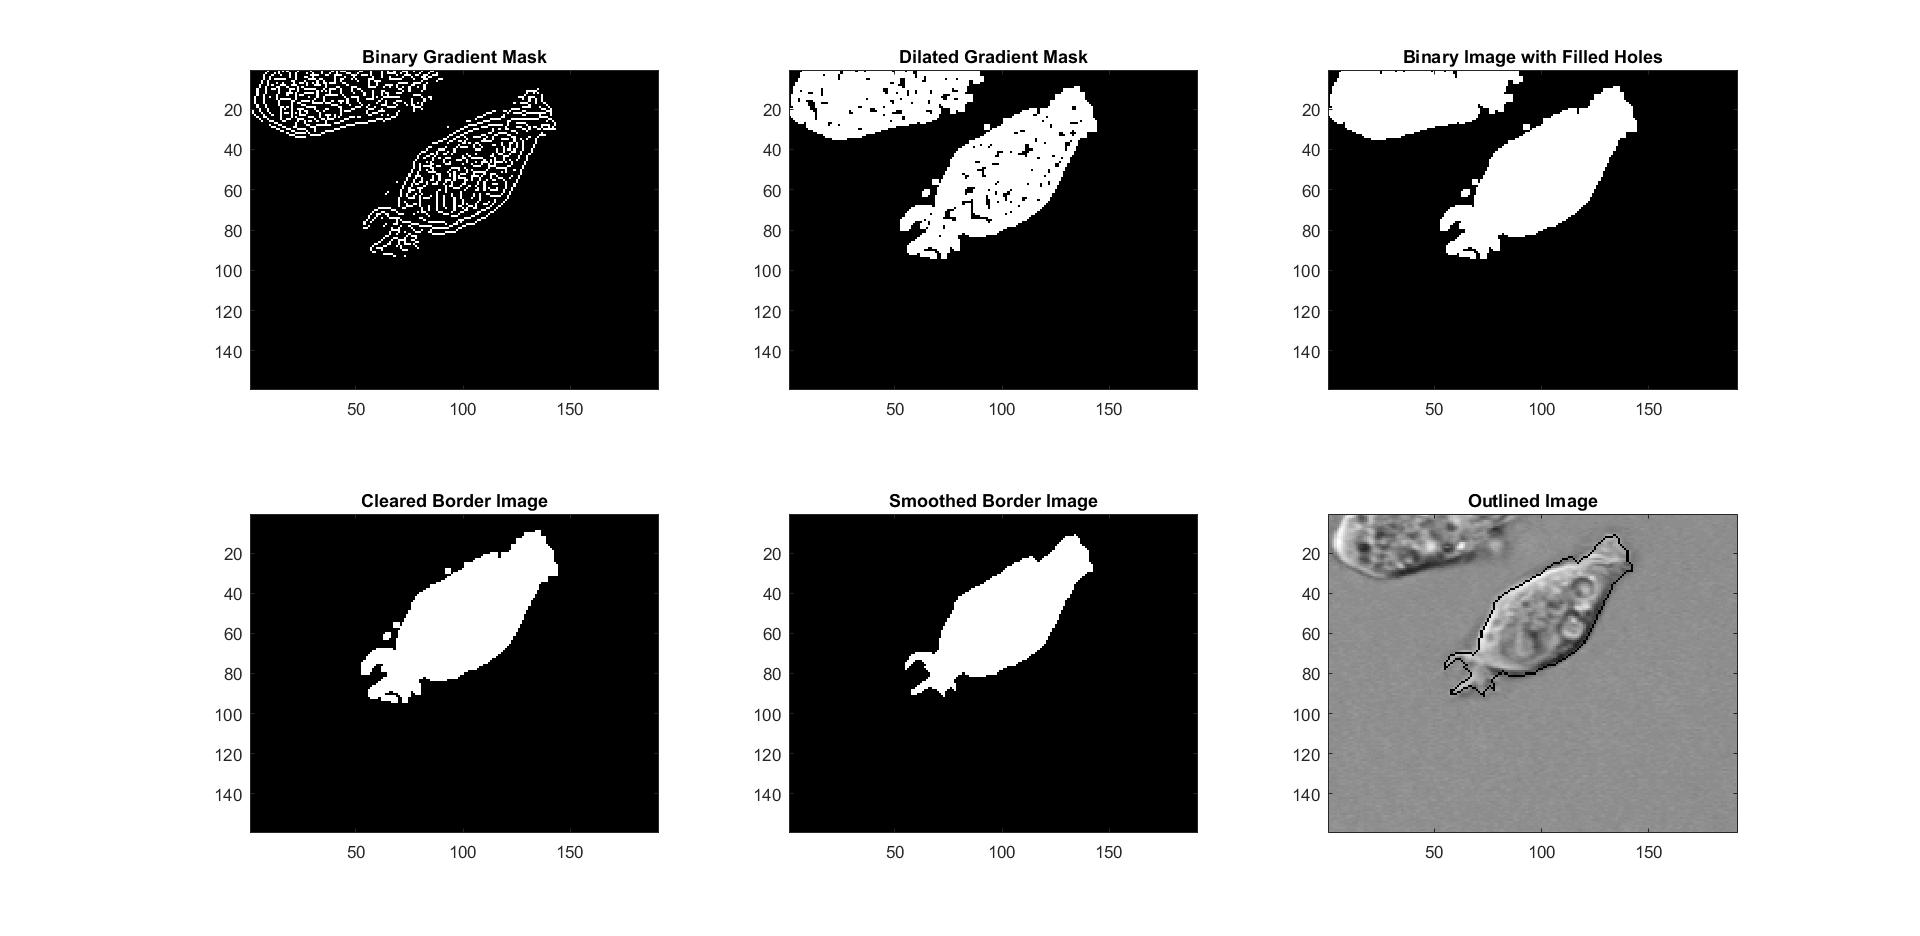
\includegraphics[height=\linewidth, width=\linewidth]{./output_images/lab5_results.jpg}
	\end{figure}
	
\pagebreak

\end{document}
